\chapter{统计学习与数据模式：常见陷阱}
\label{chap:data-patterns}

\begin{keybox}[训练目标只看见经验分布]
模型最终学到什么由数据分布、目标函数和采样过程共同决定。这里把前文所有模型重新放回同一个审计闭环：训练集是否代表部署分布，loss 是否奖励真正关心的性质，生成器是否覆盖模式与尾部，服务中的筛选和合成数据回流是否悄悄改变下一轮经验分布。
\end{keybox}

\section{数据分布比数据总量更重要}

若训练集由多个来源混合而成，经验分布其实是 \(\hat\pi=\sum_k\alpha_k\hat\pi_k\)。改变比例 \(\alpha_k\) 就改变了被优化的目标，即使总 token 数不变。科学数据还经常存在温度、压力、相区、几何尺寸或实验设备的分层结构；逐样本随机切分时，同一次实验或模拟的相邻记录可能同时进入训练和测试，使测试结果偏乐观。若反复把模型生成的数据用于后续模型的训练，而缺少真实数据校正，稀有模式还可能逐轮减少~\cite{shumailov2024curse}。

\begin{table}[ht]
\centering\small
\begin{tabularx}{\textwidth}{>{\bfseries}p{29mm} X X}
\toprule
数据模式 & 可能后果 & 验证项目\\
\midrule
长尾 & 高频 token 主导平均 loss；占 2\% 的稀有模式在平均 NLL 中也只占 2\% 权重 & 按频率、领域、长度、语言和任务分层报告\\
重复/污染 & 验证 loss 与 benchmark 被高估，记忆被误判为推理；相邻帧的相似度可以接近 1 & 近似去重、时间切分、训练-测试相似度审计\\
混合分布 & 模型学到来源比例和格式偏差 & 保存来源标签，报告每个子分布指标\\
轨迹相关 & 同一实验或模拟的相邻状态高度相似；逐样本随机切分会让测试结果偏乐观 & 让同一对象或整条轨迹只进入一个数据集；预测未来时按时间切分\\
非平稳 & 数据分布随时间变化，未来数据与训练数据不同，旧测试结果可能失效 & 按时间留出较新数据，记录条件变化，持续监测模型表现\\
合成递归 & 反复用上一代模型生成的数据训练下一代，稀有模式可能逐轮减少，错误可能累积 & 保留真实数据，记录生成器、筛选规则与合成比例，并检查稀有模式\\
\bottomrule
\end{tabularx}
\caption{数据审计应围绕分布结构展开，样本数量只是其中一项。}
\label{tab:data-patterns}
\end{table}

“轨迹相关”例如：同一分子动力学轨迹的相邻帧很相似。若分别放入训练集和测试集，模型可能靠识别近似重复的状态得分，未必能预测新轨迹。评估新轨迹时，应将整条轨迹只放入训练、验证、测试中的一组；评估未来状态时，按时间切分，并避免相似帧跨组。

“非平稳”指数据的统计分布随时间改变。例如，用某实验装置上半年的测量训练模型，后来更换传感器或调整工作温度，下半年的读数范围和噪声水平可能变化。即使模型在随机抽出的历史测试集上表现很好，也未必适用于新条件。应留出较晚时间段的数据单独测试，按设备和实验条件分层报告，并在部署后检查输入分布及模型误差是否变化。

“合成递归”是指模型 A 生成样本训练模型 B，模型 B 再生成样本训练模型 C，如此反复。如果每轮生成或筛选都漏掉少见的样本，下一轮的训练数据就更缺少这些样本，模型可能越来越不擅长生成它们。若每一轮丢掉 10\% 的稀有模式，十轮后只剩约 \(0.9^{10}\approx0.35\)。风险大小取决于合成数据的质量和占比、筛选方式，以及每轮是否继续加入足够的真实数据。

\section{训练与采样的错位}

teacher forcing 在第 \(t\) 步使用真实的 \(x_{<t}\)，但部署时模型接收到的是自己采样的前缀。一个小的局部错误会改变后续条件分布，形成 exposure bias。缓解办法包括 scheduled sampling~\cite{bengio2015scheduled}、数据增强、从模型生成的轨迹上训练、搜索/验证、过程监督和更强的后训练；这些方法都会改变统计目标，比较时应在同一目标下进行。

\section{似然、样本质量与模式覆盖}

判别式分类有真实类别标签，受试者工作特征曲线下面积（area under the receiver operating characteristic curve，ROC-AUC）等指标可以概括模型区分正负样本的能力。ROC-AUC 汇总了不同判别阈值下的表现。生成模型通常没有一个被广泛接受、又能同时概括主要性能维度的单一指标，因此评价往往比分类更复杂。即使在图像生成中，弗雷歇 Inception 距离（Fréchet Inception Distance，FID）等自动指标也难以充分判断视觉自然度、局部瑕疵或内容是否符合条件；许多实际比较仍需要人眼评审。

评价生成模型要分别回答：模型给真实测试样本多大概率；从模型抽出的单个样本是否可信或有用；大量生成样本能否覆盖真实分布的不同模式及长尾。似然或负对数似然（NLL）回答第一个问题。较高的测试似然说明模型对已观测数据分配了较多概率质量；单张样本是否自然、采样温度与引导是否合适，需要另外的指标。高维图像模型中，平均对数似然与视觉保真度可以相当独立~\cite{theis2016evaluation}。

反过来，生成样本看起来很好，也可能只来自真实分布的一小部分。设真实数据有几种不同的构象或图像类别，一个生成器只产生其中最容易的一类，每个样本都很逼真，但其他模式的概率几乎为零；这就是\textbf{mode collapse（模式坍缩）}。采样时只保留高分结果也可能提高单样本质量，同时丢掉多样性。因而至少要分别报告\textbf{保真度}与\textbf{覆盖度}，并针对稀有模式或物理相区单独检查，不能让一个平均分数代替所有结论。

\Needspace{10\baselineskip}
\section{常见生成指标各自在测什么}

为了避免把“拟合真实数据”“单张样本可信”和“覆盖全部模式”混成一个分数，下面分别说明常用指标的比较对象。

下表中的困惑度（perplexity，PPL）用于评价语言模型。这里的 Inception 特征是指：将图像输入在 ImageNet 上预训练的 Inception-v3 分类网络，取分类层之前的中间激活向量（通常取最后的全局平均池化层输出），作为这张图像的数值表示。FID 先把真实图像和生成图像分别变成这样的特征向量，再比较两组向量的均值和协方差；因此它衡量的是选定特征空间中的整体统计差异。

\begin{table}[ht]
\centering\small
\begin{tabularx}{\textwidth}{>{\bfseries}p{34mm} X X}
\toprule
指标 & 实际比较的对象 & 主要局限\\
\midrule
测试集 NLL / PPL & NLL 是真实测试样本的平均负对数概率；PPL 是平均 token NLL 的指数 & 衡量给真实数据的概率，不直接衡量抽样文本是否有用；不同数据集或 tokenizer 的 per-token 数值不宜直接比较\\
FID & 比较真实图像与生成图像在 Inception 特征中的均值和协方差，越低表示这两个统计摘要越接近 & 把保真度与覆盖度混在一个数里；依赖特征网络、预处理和样本数，不能保证局部模式都被覆盖\\
Precision/Recall & 在特征空间中，Precision 估计生成样本靠近真实区域的比例；Recall 估计真实区域被生成样本覆盖的程度 & 能分开观察样本质量与覆盖度，但依赖特征表示、邻域定义及样本量\\
\bottomrule
\end{tabularx}
\caption{三个常用指标分别观察概率拟合、图像特征统计，以及生成样本的保真度和覆盖度。FID 与生成模型 Precision/Recall 的定义见相应原始工作~\cite{heusel2017fid,kynkaanniemi2019precisionrecall}。}
\label{tab:generation-metrics}
\end{table}

对自回归语言模型，若测试集共有 \(N\) 个被计分 token，\(\mathrm{PPL}=\exp\!\bigl[-N^{-1}\sum_t\log p_\theta(x_t\mid x_{<t})\bigr]\)。所以 PPL 只是把平均 token NLL 换一个尺度；长回答是否重复、事实是否正确、条件是否满足，需要另外检查。FID 与生成模型的 Precision/Recall 主要用于图像；在分子或物理构型上，应改用与对象相关的结构描述和观测量。

\section{校准与分布外泛化}

对条件生成还要检查生成结果是否满足给定条件；对科学数据还要检查守恒律、对称性和有效结构。校准问题可以问：模型给出 0.8 的事件概率时，长期频率是否接近 0.8？OOD（Out-of-Distribution，分布外）问题可以问：模型在远离训练支撑集时是否仍给出过高置信度？这两个问题都不能由单一平均 NLL、FID 或样本外观解决。

\Needspace{9\baselineskip}
\section{变分训练的诊断}

\begin{itemize}
  \item VAE：记录 reconstruction、KL、每维 KL、潜变量互信息和 posterior samples。
  \item Flow：检查 log-det 的数值范围、逆变换误差、尾部样本和 Jacobian 条件数。
  \item Diffusion：按噪声时间或信噪比分层报告 denoising loss，检查采样步数、solver、guidance 和 OOD。
  \item EBM：检查 MCMC 的自相关、有效样本数、不同初始化的混合、能量与物理量之间的关系。
  \item 自回归：检查长度分层 loss、token 频率、校准、重复率、temperature/top-$p$ 敏感性和长程一致性。
\end{itemize}

\section{物理与科学数据的额外约束}

如果数据具有群对称性，应使用 invariant/equivariant 架构或在数据/损失中明确处理；如果生成对象必须满足约束，应使用参数化保证、投影、惩罚、条件变量或后验筛选。对 Boltzmann 任务，须分别报告结构有效率、能量分布、温度、自由能差、相关函数和模式覆盖；“样本看起来像”只是最低层证据。

\begin{figure}[ht]
\centering
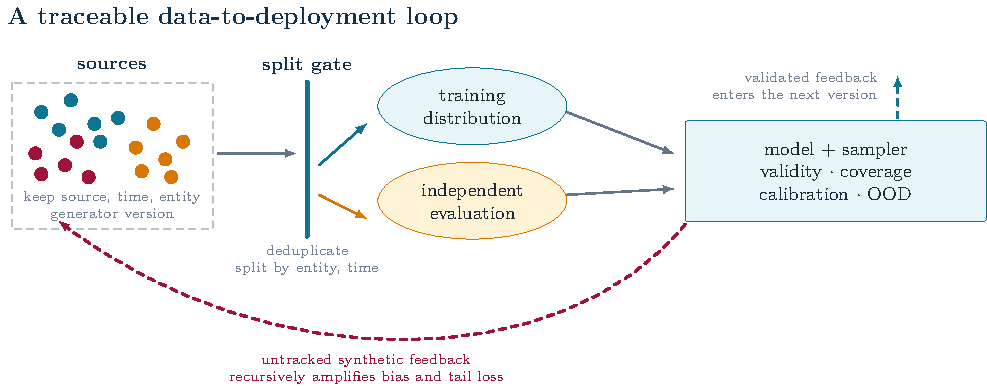
\includegraphics[width=\textwidth]{data_audit_loop.pdf}
\caption{审计闭环必须保留“样本来自哪里、如何切分、在哪个分布上评价、哪些生成样本被回流”四类信息。只有通过独立分布评估和物理约束的输出才能有条件进入下一版数据；无标记回流会把偏差和尾部丢失递归放大。}
\label{fig:audit-loop}
\end{figure}
